\documentclass[a4paper]{article}
\usepackage{graphicx}
\usepackage[hidelinks]{hyperref}
\usepackage{xcolor}
\usepackage{url}
\usepackage{outlines}
\usepackage{listings}
\usepackage{fontspec}
\lstset{basicstyle=\ttfamily,
	showstringspaces=false,
	commentstyle=\color{blue},
	keywordstyle=\color{pink}
}
\lstset{emph={
	EXPOSE,RUN,FROM,CMD,nc,tcp,udp,http,docker},emphstyle=\color{purple}
}
\newcommand{\abc}{\hfill \break}
\usepackage{fancyhdr}
\usepackage{geometry}
\geometry{
	a4paper,
	total={170mm,257mm},
	left=20mm,
	top=20mm,
	bottom=39mm,
}

\setlength{\headheight}{82.70538pt}

\fancypagestyle{oida}{
	\fancyhf{}
	\fancyhead[L]{\fontsize{7.5}{7.5}htl donaustadt\\ Donaustadtstraße 45\\
		1220 Wien\\~\\ Abteilung: Informationstechnologie\\ 
	Schwerpunkt: Netzwerktechnik}
	\fancyhead[R]{
\includegraphics[scale=0.45]{images/logo.png}}

	\fancyfoot[L]{\today}
	\fancyfoot[C]{\jobname}
	\fancyfoot[R]{Page: \thepage}
}

\begin{document}
\bibliographystyle{IEEEtran}
\pagestyle{oida}
\section*{Ethical hacking of a CTF-VM}
\par\noindent\rule{\textwidth}{0.4pt}

Laboratory protocol
Exercise 7: Ethical hacking of a CTF-VM

\begin{figure}[h]
	
\includegraphics[scale=0.5]{images/menheraMagnifier.png}
	\centering
	\caption{Grouplogo}
\end{figure}

\vspace*{\fill}
Subject:	ITSI

Class:	3AHITN

Name:	Stefan Fürst, Justin Tremurici

Groupname/number Name here/12

Supervisor: 	SPAC, ZIVK

Exercise dates:	

Submission date:


\newpage
\tableofcontents

\newpage

\section{Task definition}



\section{Summary}

\newpage

\section{Complete network topology of the exercise}

\newpage

\section{Exercise Execution}
\subsection{Setting up the virtual machines.}
To get started with this CTF, make sure that VirtualBox version 7.1.4 is used. The VM to attack must be imported by double-clicking the provided \texttt{.ova} file. After the import is complete, the network settings must be changed to use Host-only Adapter mode. Since using the default Host-only network did not work, we had to create a new Host-only network. To do this, either press \texttt{<C-h>} or click on \texttt{File} > \texttt{Tools} > \texttt{Network Manager}, as shown in Figure 2.
\begin{figure}[h]
	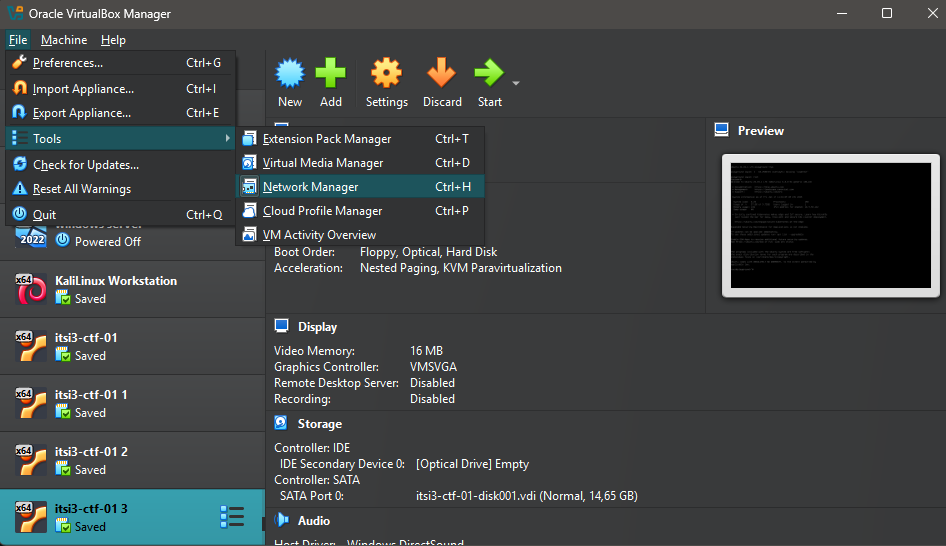
\includegraphics[scale=0.285]{./images/openingNetworkManager.png}
	\centering
	\caption{Opening VirtualBox Network Manager settings}
\end{figure}\abc
In this menu, click on \texttt{Create}, then check the \texttt{Enable Server} box to enable the DHCP server so the target VM will receive an IP address. Then, click on \texttt{Adapter} to view the IP range of the network, which in our case is \texttt{192.168.15.0/24}, which can be seen in Figure 3.
\begin{figure}[h]
	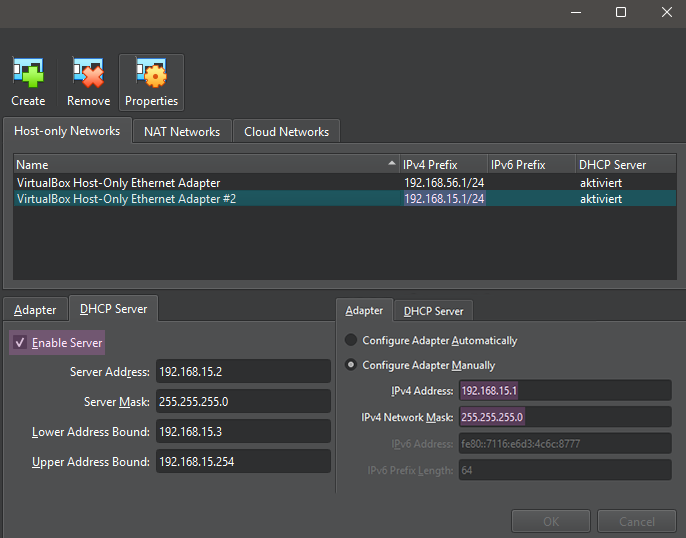
\includegraphics[scale=0.4]{./images/nwipsfr.png}
	\centering
	\caption{Showing the IP settings for the new Host-only network}
\end{figure}\abc
Next, open the virtual machine settings by selecting the VM in the list and pressing \texttt{<C-s>}. Under the \texttt{Network} section, change the network adapter to use the Host-only Adapter and select the VirtualBox Host-only Ethernet Adapter \#2, which was just created. Perform this step for both the target VM and the Kali VM, as detailed in Figure 4.
\begin{figure}[ht]
	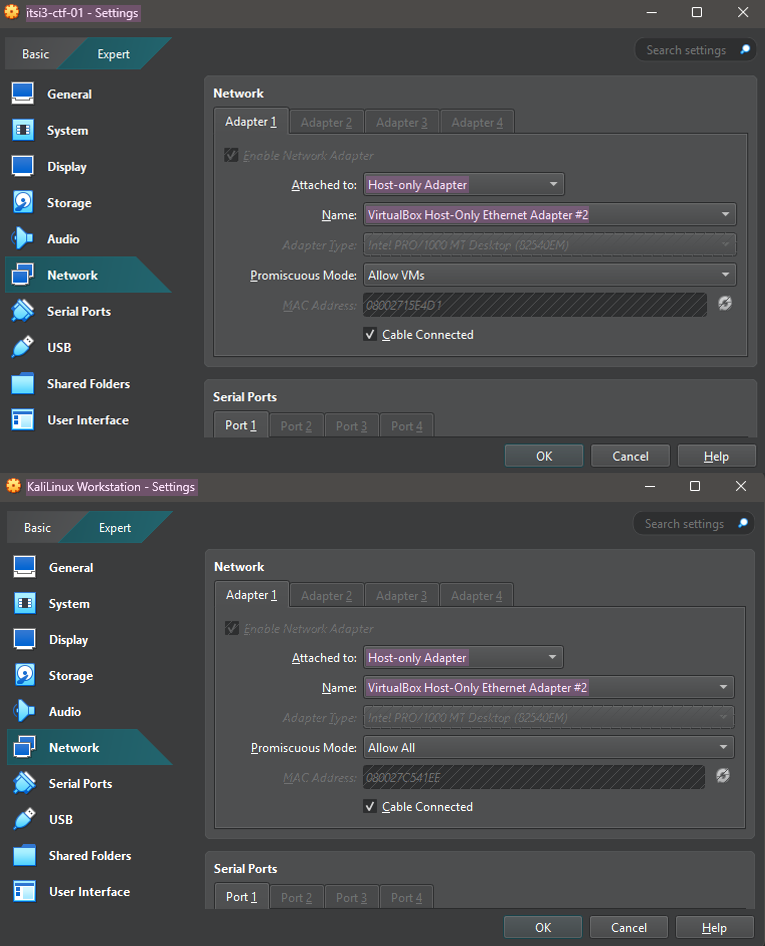
\includegraphics[scale=0.4]{./images/vmnwconf.png}
	\centering
	\caption{Showing the network configuration of the virtual machines}
\end{figure}\abc
\newpage
\subsection{Reconnaissance: Scanning the Network}
Any attack starts with recoonaise which in this case means scanning the network with \texttt{nmap} since we dont know the ip addres of the target server yet we have to scan the netowrk to find it for this the command \texttt{nmap 192.168.15.0/24} is used to scan the entire network for open ports.
\subsection{exploring the websites}
\subsection{breaking the http authtication}
\subsection{sshing into the server}
\subsection{exploring the system}
\subsection{procces flag}
\subsection{comment flag}
\subsection{sudo flag}
\subsection{history flag}
\subsection{tmp flag}
\subsection{it's over but actually not}
\subsection{trying to escalate privaledgs}
\subsubsection{smart enumeration}
\subsubsection{trying a kernel level exploit}
\subsubsection{checking suid binarys}
\subsubsection{checking root proccses}
\subsubsection{trying metasploit}
\subsubsection{trying other common ctf priv escalation ways}
\subsection{reseting the root password and exploring the vm}
\subsection{7 flags}
\subsection{talking abt the setup etc or sum idk :shruge:}

\newpage
\section{References}
\bibliography{IEEEabrv,quellen}
\newpage
\section{List of figures}

\listoffigures

\end{document}
